\begin{exo}{}
	On considère le tableau de variations d'une fonction $f$.

	\vspace*{2mm}
	\begin{center}
		\begin{tikzpicture}
			\tikzset{arrow style/.style={->, >=Triangle, thick}}
			\tkzTabInit[lgt=1, espcl=1.5]{$x$ / 0.7 , $f$ / 1.3}{$-\infty$, $-3$, $4$, $7$}
			\tkzTabVar{-/ , +/ $4$, -/ $-1$, +/ $3$}
		\end{tikzpicture}
	\end{center}
	\begin{enumerate}
	\item Déterminer l'ensemble de définition $\mathcal{D}$ de $f$ puis décrire les variations de cette fonction sur $\mathcal{D}$
	\end{enumerate}
\end{exo}
